\section{Transfer between halos}
\label{sec:transfer}

Now that we have fully considered our particle-level metric, which has shown
that dark matter and baryons in the \simba{} cosmological simulations have
vastly different dynamics, let us move on to considering the movement of
baryons between bound structures. The below analysis considers the transfer
of baryons between halos and their associated lagrangian regions. For our
definitions of these, please see \S \ref{sec:simba}.

\subsection{The different origins of baryonic and dark matter}

% For bigtransferpic please see feedbackmetrics.tex.

Figure \ref{fig:bigtransferpic} shows simultaneously the initial and final
states of the simulation, with the main purpose of this figure being to show
the mixed origins of the gas and dark matter in bound structures at redshift $z=0$.
A common trend for all halos is a shell of gas around the main dark matter component
in the initial conditions, showing that gas in general is able to collapse
further (due to cooling) than the dark matter, which is unable to lose angular
momentum as efficiently. This corresponds to the slightly further mean spread metric
for halo gas shown in Figure \ref{fig:distbaryon} than dark matter resident in
halos.

Note that the origin of the dark matter in the initial conditions corresponds
exactly to our definition of lagrangian region for that component in \S \ref{sec:simba}.
These lagrangian regions have very complex shapes, with them becoming more complex with
lower halo mass (as objects become less powerful attractors) and increasing amounts
of transfer (see below). These non-spherical shapes are why we chose to identify
our lagrangian regions for gas in the way that we did (i.e. through neighbour searching,
rather than through a fixed 3D aperture), as anything else would leave us unable to 
capture the surprisingly intricate structure that is at play here.


\subsection{Calculating transfer between lagrangian regions}

Now that the lagrangian regions have been defined, it is possible to consider on
a particle-by-particle basis where particles started and where they ended up.
The algorithm is as follows:
\begin{enumerate}
	\item ID match all particles between the initial and final conditions, including
	      star particles (these are matched to their gas progenitor). Black holes
	      are ignored in this analysis.

	\item Every particle in the $z=0$ final conditions has several possible final
	      states and origins, based on its halo ID $i$:
	      \begin{itemize}
	            \item Particle resides in a halo $i$
	            \begin{itemize}
	           		\item Particle originated in the same lagrangian region $j = i$
	           		\item Particle originated outside any lagrangian region $j = -1$
	           		\item Particle originated in some other lagrangian region $j \neq i$
	            \end{itemize}
	            \item Particle resides outside a halo ($i = -1$)
	            \begin{itemize}
	            	\item Particle has never been in any lagrangian region or halo
	            	\item Particle originated in a lagrangian region $j$ and was moved out
	            \end{itemize}
	      \end{itemize}
	      
	\item For every halo and lagrangian region the mass originating from each
	      of the above components is computed and stored.
\end{enumerate}

% for lrtransfer see feedbackmetrics.tex

A visualisation of the results of this process is shown in Fig. \ref{fig:lrtransfer},
split by four main lagrangian components that we will be considering in the
remainder of this paper. Considering each panel clockwise from the top left
we see first the gas that is in the same halo as the dark matter that resides there.
Here, we see points corresponding to every halo in the box in characteristic (for
AHF) spherical shapes. The centers of these spheres, where the gas is densest,
are the brightest.

Second we have the gas that is outside any halo at redshift $z=0$, but is assigned
to a lagrangian region; this is the gas that `should' have ended up in the halos by
the end of the simulation. We see that this gas traces the large-scale bubbles that
the AGN power, with some of this gas piling up just outside the virial radius for
the halos. A lot of this gas lives in filaments, but very little in of it resides
in voids.


The gas that is always outside any lagrangian region traces the majority of the
filamentary structure, and shows all of the structure in the voids. This is
gas whose initial closest neighbour also resides outside of a halo at redshift
$z=0$ (approximately half of the dark matter).

Finally we have the gas that is in halos but from outside any lagrangian
region. This shows a very similar structure (albeit less bright) to the gas
that resides in its own halo, but it originated from a region where the dark
matter now resides outside of a halo. This gas is likely dragged into these
bound structures by cooling flows, while the dark matter is not able to lose
angular momentum quickly enough to assemble by $z=0$.


\subsection{Transfer in a non-radiative Model}

\begin{figure}
	\centering
	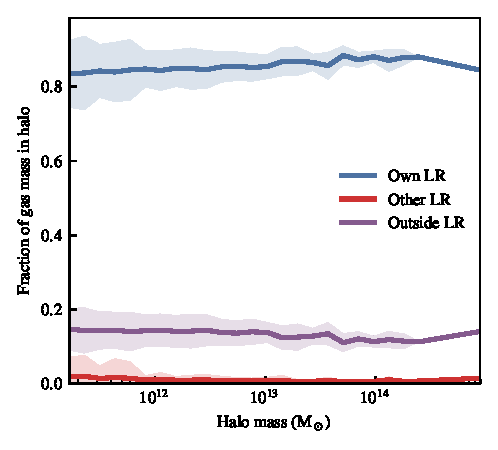
\includegraphics[width=\columnwidth]{figures/s50gadget/component_fraction_vs_halo_mass_gas.pdf}
	\vspace{-0.7cm}
	\caption{
	The fraction of baryonic mass originating from each lagrangian component is
	shown as a function of redshift $z=0$ halo mass, later referred to as the
	Baryon Transfer Mass Function (BTMF). This is only provided for comparison to
	the full model result in Fig. \ref{fig:maintransferresult}.
	}
	\label{fig:nonradiativetransfer}
\end{figure}

Now that we have seen the significant differences in the spatial distributions
of gas in various lagrangian components, let us see if there are any trends
with halo mass.

To begin with, let us consider a null model. In this case, we run the
simulation in non-radiative mode; i.e. without cooling, star formation, or
feedback. This simulation only includes hydrodynamics, cosmology, and
gravity. In Fig. \ref{fig:nonradiativetransfer} we present the fraction of
baryonic mass for each halo contributed from each lagrangian component, as a
function of halo mass. There is no dependence on halo mass (as the simulation
is effectively scale-free above some resolution limit), and apart from some
small level of transfer from outside any lagrangian region, the baryonic mass
in each halo consists of that which originated in its own lagrangian region.
This difference, as described in \S \ref{sec:feedbackmetrics}, is likely
caused by gas that piles up on the outside of each halo due to accretion
shocks while the collisionless dark matter is stripped by passing straight
through or around the bound structure

\subsection{Transfer \emph{into} halos in \simba{}}

\begin{figure*}
	\centering
	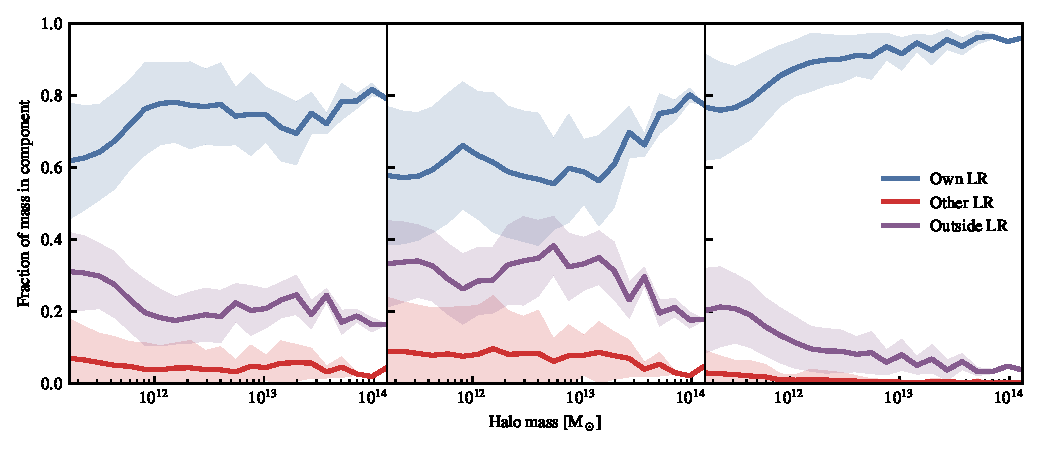
\includegraphics{figures/s50j7kAHF/component_fraction_mixed.pdf}
	\vspace{-0.7cm}
	\caption{
		The fraction of baryonic mass originating from each lagrangian component is
		shown as a function of redshift $z=0$ halo mass, later referred to as the
		Baryon Transfer Mass Function (BTMF). Different panels show different
		particle selections with all baryonic
		mass (left), gas mass (center), and stellar mass (right). Shaded
		regions show the $1\sigma$ scatter in a given bin, with one standard
		deviation of variation being shown. There is no attempt made to include
		halo assembly bias or the finite halo sampling in a $50\hmpc{}$ box in
		these regions.
	}
	\label{fig:maintransferresult}
\end{figure*}

The results of the full model, transfer as a function of halo mass, are shown
in Fig. \ref{fig:maintransferresult}. The general trend is that for an
increasing halo mass, a lagrangian region is able to hold on to more of the
original baryonic mass, with this flattening off around $M_H = 10^{12}
\msolar$. For a given halo, significantly more of the gaseous mass originates
outside the original lagrangian region as compared to the stellar mass ($\sim
40 \%$ versus $\sim 10 \%$). The transfer between halos is at around the
$\sim 10\%$ baryonic mass level, with this transfer predominantly
originating from the gaseous component, as compared to the stellar component.
This combines nicely with the distance metrics shown in \S
\ref{sec:feedbackmetrics}, which showed that the dark matter and stars have
very similar dynamics and hence should be similarly well bound.

This transfer can have several physical origins. The first, as shown in the
non-radiative run, is caused by the collisional dynamics of the gas preventing
gas from following the dark matter in all cases. We see that this can account
for up to 15\% of the baryonic mass of a bound structure at redshift $z=0$ originating
from a different region than the dark matter, but this could not account for any
\emph{inter-lagrangian} region transfer.

The galaxy formation sub-grid model clearly has a significant effect on the 
baryonic make-up of halos at redshift $z=0$. The fraction of mass from outside
any lagrangian region have increased to 20-40\% (it is unclear whether we should
compare the total baryonic component or the gaseous component to the non-radiative
run). This increase is explained by the inclusion of sub-grid cooling, with particles
now able to form cool accretion flows that can lose angular momentum at a much higher
rate than the dark matter component is able to.

Around 10\% of the baryonic mass of halos is now made up of gas that has
experienced inter-lagrangian transfer. It is important to recall that this is transfer
between bound structures at redshift $z=0$, and that it only takes into account
the initial and final conditions of the simulation; we do not know the complete history
of these particles.


The transfer has several possible sources: stripped gas from nearby galaxies that are
still classified as their own bound structures at redshift $z=0$, gas that has 
been expelled from galaxies through stellar winds or AGN feedback and re-captured
by a halo, and spurious transfer in the initial conditions due to the way that
we have classified our lagrangian regions. With the non-radiative simulation
showing zero transfer between bound structures, and there being little transfer
before redshift $z=2$, we believe that the contribution from this component is
likely very small. Turning off the AGN winds reduces this transfer by a small amount,
but it still remains at the 10\% level as shown here; if this transfer
is powered by feedback events it must be dominated by the expulsion
(or preventative feedback) from stellar winds.

A given mass bin contains halos that entertain a range of 10x in transfer,
which is likely dependent on environment as shown in Figure
\ref{fig:bigtransferpic}. The specific physical effects that lead to the
scatter in these relations will be discussed in a follow-up paper.

The overall fraction of baryonic mass that is retained by a given lagrangian
region does begin to turn over around $10^{13} \msolar{}$, however it is unclear
whether this is due to a lack of higher mass halos in the $50 \hmpc{}$ box. It
is also important to note that the shaded regions in Figure
\ref{fig:maintransferresult} represent the $1\sigma$ scatter in a given bin
and explicitly do \emph{not} include any errors that would occur from a finite
sampling of halos or halo assembly bias.

\subsection{Transfer \emph{out} of Lagrangian Regions}

\begin{figure}
	\centering
	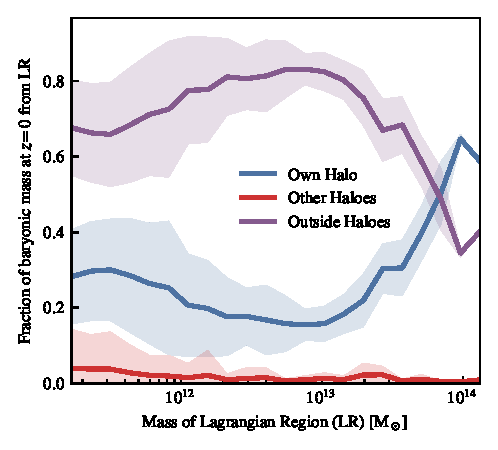
\includegraphics{figures/s50j7kAHF/inverse_component_fraction.pdf}
	\vspace{-0.7cm}
	\caption{The fate of gas that begins in lagrangian regions, as a function of
	initial lagrangian region mass. This shows the impact of AGN
	feedback with the dip between $10^{12}\msolar{}$ and $10^{13}\msolar{}$
	representing an overall ejection of baryons as this pathway
	becomes efficient. The peak at just below $10^{12}\msolar{}$
	for retained gas corresponds to the halo mass where AGN feedback
	and stellar feedback are both relatively inefficient.}
	\label{fig:transferoutoflrs}
\end{figure}

The clear inverse to the above discussion is to consider what happens to the gaseous
material that originated in a given lagrangian region. Now looking at the results as
a function of lagrangian region mass (this is slightly higher than the eventual
halo mass as the baryon fraction of a given halo is lower than the cosmic mean), it
is clear that there is an even more significant transfer \emph{out} of lagrangian
regions than \emph{into} halos (see Figure \ref{fig:transferoutoflrs}). Only 
approximately $20\%$ of the gas initially resident in a given lagrangian region
makes it into the $z=0$ halo. The more massive halos in the box (of which there 
are very few) manage to accrete the majority of the baryons associated with their
lagrangian region.

The relation between halo mass and transfer out of the lagrangian region peaks
around $10^{12.5-13}\msolar{}$ where the efficiency of AGN feedback peaks. What
is surprising, though, is that this AGN feedback is more effective at evacuating
baryons from intermediate mass halos than stellar feedback is at evacuating
baryons from low mass halos. This is because preventative feedback also has
significant effects here, with accretion impacted by the hot IGM and CGM that
surrounds the galaxies in these halos.

\begin{figure}
	\centering
	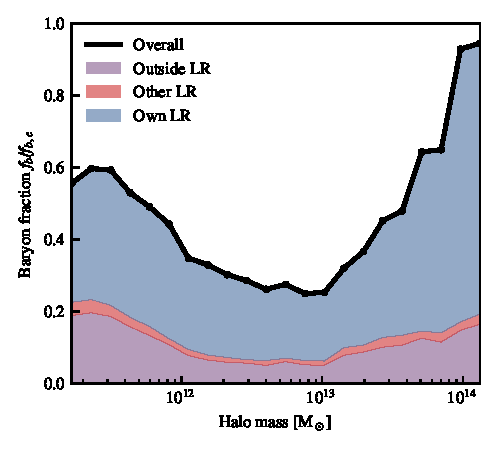
\includegraphics{figures/s50j7kAHF/baryon_fraction_breakdown.pdf}
	\vspace{-0.7cm}
	\caption{The baryon fraction $f_b$ relative to the cosmic baryon fraction
	$f_{b, c}$ shown as a function of halo mass. The coloured bands show the
	contributions to the baryon fraction from various lagrangian components.}
	\label{fig:baryonfraction}
\end{figure}

The baryon fraction of the $z=0$ halos in Figure \ref{fig:baryonfraction}
shows, as expected, a strong dependence on halo mass ($M_H$). Halos with a
mass  $M_H > 10^{12} \msolar{}$ can have efficient AGN feedback; this has two
effects. The AGN feedback causes a the halo to become heated to $T_{\rm
vir}$, the virial temperature of the halo (typically $\sim10^{7-8}$ K for Milky
Way-mass halos). This `hot halo' acts to prevent infall from outside, a
clearly efficient pathway in \simba{} as the halo since infall from outside of
the lagrangian region is curtailed by 50\% in this mass region.  The other
pathway is to eject mass that was already inside the lagrangian region; this
effect is less powerful in \simba{} as gas from the lagrangian region of the
halo is only affected at the $\sim10-20\%$ level.

Once halos begin to reach $M_H > 10^{14} \msolar{}$, the potential well
becomes too deep and so the evacuation caused by AGN feedback again stops
being efficient, causing a significant increase in the retention of baryons
that originated from that halo's lagrangian region. The dependence of baryons
accreted from outside of any lagrangian region on halo mass appears to be
relatively weak, with a much less significant dip at $10^{12} \msolar{} < M_H
< 10^{14} \msolar{}$.
